\documentclass[10pt]{beamer}

\usetheme{m}

\usepackage{booktabs}
\usepackage[scale=2]{ccicons}

\title{Deduction as a Service}
\subtitle{}
\date{\today}
\author{Mohamed Bassem}
\institute{German University in Cairo}

\begin{document}

\maketitle

\begin{frame}
  \frametitle{Table of Contents}
  \setbeamertemplate{section in toc}[sections numbered]
  \tableofcontents[
    hideallsubsections,
  ]
\end{frame}

\section{What is E?}
\begin{frame}[fragile]
  \frametitle{What is E?}

  E is a theorem prover that takes a set of axioms and tries to derive a formal proof to a given conjuncture

  \pause{}
  Example:
  \begin{figure}
    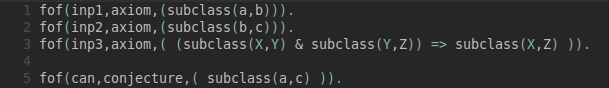
\includegraphics[width=90mm]{imgs/SampleAxioms.png}
  \end{figure}
\end{frame}


\section{Large Axiom Sets}
\begin{frame}[fragile]
  \frametitle{Large Axiom Sets}
\end{frame}


\section{Problem}
\begin{frame}[fragile]{Only}
  \frametitle{Problem}
  \begin{itemize}
    \item<only@1,3>Running multiple queries against the same knowledge base requires re-parsing the whole set

    \item[]<only@2> \begin{figure}
        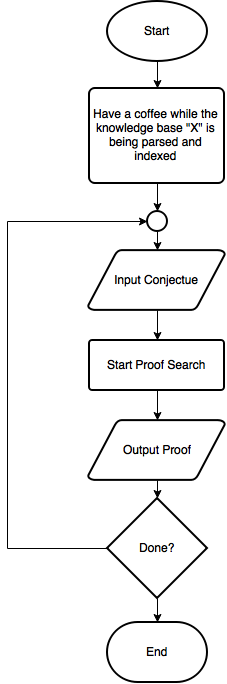
\includegraphics[width=\linewidth,height=\textheight,keepaspectratio]{imgs/NewDeductionFC.png}
      \end{figure}
    \item<only@3>\alert<3>{No formal way of communicating with E other than invoking the executable}
  \end{itemize}
\end{frame}

\section{Solution}
\begin{frame}[fragile]
\frametitle{Solution}
  \begin{itemize}
    \item<only@1,3,4> Sessions
    \item<only@2> 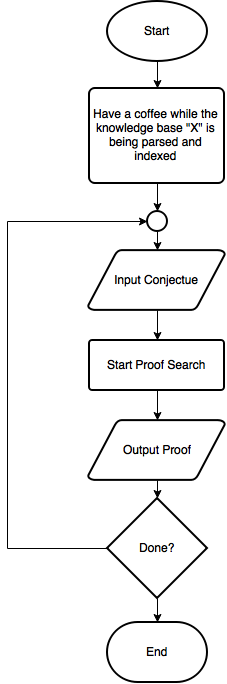
\includegraphics[width=\linewidth,height=\textheight,keepaspectratio]{imgs/NewDeductionFC.png}
    \item<only@3,4> \alert<3>{Server Client Architecture}
    \item<only@4> \alert<4>{Interaction Protocol}
  \end{itemize}
\end{frame}

\section{Benchmarking}
\begin{frame}[fragile]
\end{frame}

\section{Future Work}
\begin{frame}[fragile]
\end{frame}


\section{Conclusion}
\begin{frame}[fragile]
\end{frame}

\plain{Questions?}
\plain{Thank you}

\begin{frame}[allowframebreaks]

  \frametitle{References}

  \bibliography{demo}
  \bibliographystyle{abbrv}

\end{frame}

\end{document}
